\documentclass[../main-report.tex]{subfiles}
\begin{document}
\section{Tổng quan thuật toán}
\subsection{Giới thiệu}
Cây quyết định là một mô hình \textit{supervised learning} trong \textit{Machine Learning}, có thể được áp dụng vào cả hai bài toán \textit{classification và regression}. Việc xây dựng một cây quyết định trên dữ liệu huấn luyện cho trước là việc xác định các câu hỏi và thứ tự của chúng. Một điểm đáng lưu ý của decision tree là nó có thể làm việc với các đặc trưng (trong các tài liệu về decision tree, các đặc trưng thường được gọi là thuộc tính – \textit{attribute}) dạng \textit{categorical}, thường là rời rạc và không có thứ tự. Ví dụ, mưa, nắng hay xanh, đỏ, \ldots. Decision tree cũng làm việc với dữ liệu có vector đặc trưng bao gồm cả thuộc tính dạng categorical và liên tục (numeric). Một điểm đáng lưu ý nữa là cây quyết định ít yêu cầu việc chuẩn hoá dữ liệu.

\subsection{Phân loại}
Có 3 loại cây quyết định phổ biến sau:

\begin{itemize}
\item \textbf{Iterative Dichotomiser 3 (ID3)} - Tạo cây nhiều chiều, tìm cho mỗi node một đặc tính phân loại sao cho đặc tính này có giá trị ``information gain'' lớn nhất. Cây được phát triển tới mức tối đa kích thước. Sau đó áp dụng phương thức cắt tỉa cành để xử lý những dữ liệu chưa nhìn thấy.
\item \textbf{C4.5} - Kế thừa từ ID3 nhưng loại bỏ hạn chế về việc chỉ sử dụng đặc tính có giá trị phân loại bằng cách tự động định nghĩa một thuộc tính rời rạc. Dùng để phân chia những thuộc tính liên tục thành những tập rời rạc.
\item \textbf{Classification and Regression Trees (CART)} - Tương tự như C4.5, nhưng nó hỗ trợ thêm đối tượng dự đoán là giá trị số (\emph{\gls{regression}}). Cấu trúc CART dạng cây nhị phân, mỗi nút sử dụng một ngưỡng để đạt được ``information gain'' lớn nhất.
\end{itemize}

%Hình \ref{fig:decision_tree_type_comparison} so sánh giữa các loại thuật toán decision tree.
%
%\begin{figure}[ht!]
%\centering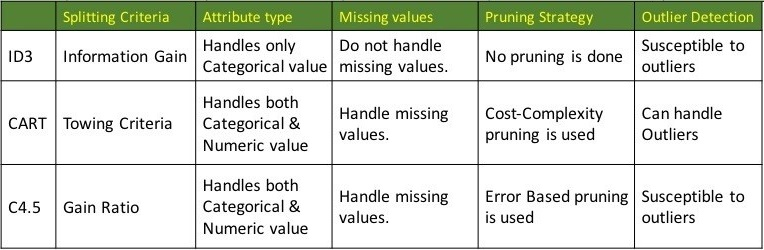
\includegraphics[scale=0.75]{comparison-decision-trees}
%\caption{So sánh các thuật toán Decision Trees}
%\label{fig:decision_tree_type_comparison}
%\end{figure}

\subsection{Ưu và nhược điểm của thuật toán}
Tùy vào loại cây quyết định mà có ưu nhược điểm riêng. Nhưng nhìn chung thuật toán có những ưu nhược điểm chung như sau:
\subsubsection*{Về ưu điểm}
\begin{itemize}
\item Cây quyết định thường mô phỏng cách suy nghĩ con người. Vì vậy mà đơn giản để hiểu và diễn giải dữ liệu.
\item Giúp nhìn thấy được sự logic của dữ liệu.
\item Có khả năng chọn được những đặc trưng tốt nhất.
\item Phân loại dữ liệu không cần tính toán phức tạp.
\item Giải quyết vấn đề nhiễu và thiếu dữ liệu.
\item Có khả năng xử lý dữ liệu có biến liên tục và rời rạc.
\end{itemize}

\subsubsection*{Về nhược điểm}
\begin{itemize}
\item Tỉ lệ tính toán tăng theo hàm số mũ.
\item Dễ bị vấn đề overfitting \footnote{\textbf{Overfitting} là hiện tượng mô hình tìm được quá khớp với dữ liệu huấn luyện dẫn đến sự nhầm nhiễu.} và underfitting \footnote{\textbf{Underfitting} là hiện tượng mô hình tìm được khác xa so với thực tế.} khi tập dữ liệu huấn luyện nhỏ.
\end{itemize}

Bài báo cáo này sử dụng loại \textbf{CART}. Do tính đơn giản và dễ tiếp cận cũng như những giá trị đặc trưng sử dụng là kiểu dữ liệu liên tục không phải phân loại nên không dùng \emph{ID3} được. Và đây là loại cây quyết định được thư viện \textit{scikit-learn} chọn sử dụng.

\subsection{Một số khái niệm}
Trước khi thực hiện xây dựng cây, ta cần giới thiệu một số hàm dùng để tính toán hiệu quả của từng bước phân chia dữ liệu trong quá trình xây dựng cây sau này.

\begin{enumerate}
\item \textbf{Mean Square Error - Sai số toàn phương trung bình}

\textbf{MSE} là thước đo để đánh giá chất lượng của một ước lượng (ví dụ, một hàm toán học lập bản đồ mẫu dữ liệu của một tham số của dân số từ đó các dữ liệu được lấy mẫu) hoặc một yếu tố dự báo (ví dụ, một bản đồ chức năng có số liệu vào tùy ý để một mẫu của các giá trị của một số biến ngẫu nhiên). Định nghĩa của một MSE khác với những gì tương ứng cho dù là một trong những mô tả một ước lượng, hay một yếu tố dự báo.

Nếu ${\hat {Y}}$ là một vector của $n$ trị dự báo, và $Y$ là vector các trị quan sát được, tương ứng với ngõ vào của hàm số phát ra dự báo, thì MSE của phép dự báo có thể ước lượng theo công thức:
$$MSE\:=\:\frac{1}{n}\sum^{n}_{i=1}(Y_{i} - \hat{Y}_{i})^{2}$$

Tức là $MSE$ là trung bình $(\frac{1}{n}\sum^{n}_{i=1})$ của bình phương các sai số $((Y_{i} - \hat{Y}_{i})^{2})$. Đây là định lượng dễ dàng tính được cho một mẫu cụ thể (và do đó phụ thuộc mẫu).

\item \textbf{Mean Absolute Error - Sai số tuyệt đối trung bình}

Trong thống kê, \textbf{MSA}(sai số tuyệt đối trung bình) là thước đo sai số giữa các cặp giá trị cùng quan sát đối với cùng một hiện tượng. Ví dụ về sự tương quan giữa $Y$ và $X$ là giữa các giá trị dự đoán so với các giá trị quan sát được, giữa thời gian ban đầu so với thời gian sau khi xảy ra hiện tương hay giữa một phương pháp đo lường này với một phương pháp đo lường khác. Khi đó, $MAE$ được tính bằng tổng sai số tuyệt đối chia cho cỡ mẫu của bộ dữ liệu:
$$MAE\:=\:\frac{1}{n}\sum^{n}_{i=1}|y_{i} - x_{i}|$$

Trong đó $y_{i}$ là giá trị dự đoán và $x_{i}$ là giá trị đúng. Do đó \textbf{MAE} là trung bình của các giá trị sai số tuyệt đối $|y_{i} - x_{i}|$ của dữ liệu.

\item \textbf{Regression criterion}

Sau khi định nghĩa 2 hàm \textit{MSE} và \textit{MSA} như trên, tiếp theo ta sử dụng 2 hàm trên để định nghĩa hàm đo độ tinh khiết giữa cách bước phân chia của cây hồi quy.

Đối với bài toán hồi quy thì kết quả đầu ra là giá trị liên tục, vậy với nút m, ta tính giá trị \textit{MSE} và \textit{MSA} của nút đó như sau:

\textbf{Min Squared Error(MSE)}
  $$\overline{y}_{m} = \frac{1}{N_{m}} \sum_{y\in Q_{m}}y$$
  $$H(Q_{m}) = \frac{1}{N_{m}}\sum_{y\in Q_{m}}(y - \overline{y}_{m})^{2}$$

\textbf{ Mean Absoluted Error(MAE) (chậm hơn nhiều so với MSE)}
$$median(y)_{m} = \underset{y\in Q_{m}}{median(y)}$$
$$H(Q_{m}) = \frac{1}{N_{m}}|y - median(y)_{m}|$$

    Cuối cùng, ta có \textit{hàm tinh khiết}(\textit{Impurity function}) được định nghĩa:
\begin{equation}
    G_{Q_{m}, \theta} = H(Q_{m}) - (\frac{N_{m}^{left}}{N_{m}}H(Q^{left}_{m}(\theta)) + \frac{N_{m}^{right}}{N_{m}}H(Q^{right}_{m}(\theta)))
\end{equation}

\item \textbf{Entropy - Độ hỗn loạn}

\textbf{Entropy}(độ hỗn loạn) là khái niệm được dùng trong vật lý, toán học, khoa học máy tính (lý thuyết thông tin) và nhiều lĩnh vực khoa học khác. Dùng để chỉ độ bừa bộn của dữ liệu.

Ta có công thức tổng quát để tính giá trị entropy như sau:

\begin{equation}
E(\mathcal{S}) = -\sum_{i=1}^n p_i \log(p_i)
\end{equation}

Với $\mathcal{S}$ là tập dữ liệu, $p_i$ là tỉ lệ các điểm dữ liệu nhãn $i$ thuộc tập $S$.

\item \textbf{Gini index} 

\textbf{Gini index} : tương tự entropy, chỉ số gini index dùng để đo độ không sạch, hỗn loạn của dữ liệu.

\textbf{Công thức tính gini index:}

\begin{equation}
\mathbf{Gini}(\mathcal{S}) = 1 - \sum_{i=1}^n p^{2}_{i}
\end{equation}

Với $\mathcal{S}$ là  tập các dữ liệu, $p_i$ là xác xuất điểm dữ liệu có nhãn loại $i$. Giá trị gini \emph{càng thấp} chứng tỏ dữ liệu càng sạch, bằng 0 tức tất cả dữ liệu điều chung một nhãn.

\item \textbf{Classification criterion}

Tương tự như hàm tinh khiết của bài toán hồi quy, với bài toán phân loại ta cũng có hàm tinh khiết tương tự:

Bài toán phân loại có đầu ra là giá trị thuộc một trong $K$ lớp, ở nút lá m, xác xuất của lớp chiếm đa số là:
\begin{equation}
    p_{mk} = \frac{1}{N_{m}} \sum_{x_{i} \in R_{m}} I(y_{i} = k)
\end{equation}

Sử dụng công thức trên, ta có công thức tính giá trị \textit{Entropy} và \textit{Gini} ở các nút là:

\textbf{Gini}:
\begin{equation}
    H(Q_{m}) = \sum_{k}p_{mk}(1 - p_{mk})
\end{equation}

\textbf{Entropy}
\begin{equation}
    H(Q_{m}) = - \sum_{k}p_{mk}log_{2}(p_{mk})
\end{equation}

Từ đó, ta có hàm tinh khiết cho bài toán phân loại là:
\begin{equation}
    G_{Q_{m}, \theta} = H(Q_{m}) - (\frac{N_{m}^{left}}{N_{m}}H(Q^{left}_{m}(\theta)) + \frac{N_{m}^{right}}{N_{m}}H(Q^{right}_{m}(\theta)))
\end{equation}
\end{enumerate}

\subsection{Quá trình xây dựng cây}
Cho N bộ dữ liệu  $(x_{i}, y_{i}), i \in [1, 2, ...N]$ với:
\begin{itemize}
\item \textbf{Dữ liệu huấn luyện} : $x_{i} = (x_{i1}, x_{i2}, ..., x_{ip})$, p là số thuộc tính(features) của từng điểm dữ liệu.
\item \textbf{Nhãn} : $y \in R^{N}$
\end{itemize}

Thuật toán cây quyết định phân chia đệ quy các thuộc tính của dữ liệu sao cho các dữ liệu có nhãn giống nhau được gộp chung lại. Cây chia bộ dữ liệu thành M vùng $R_{1}, R_{2}, ..., R_{M}$.

Mỗi điểm dữ liệu sẽ được dự đoán như sau:
$$f(x) = \sum_{i}^{M} c_{m}I(x \in R_{m})$$

Với bài toán hồi quy (Regression), $c_{m}$ được tính là trung bình của giá trị ở nút lá của tất cả điểm dữ liệu. Với bài toán phân loại(Classification), $c_{m}$ được tính dựa vào lớp có lượng đông nhất ở các nút lá.

Thuật toán cây quyết định chia dữ liệu thành các vùng để xây dựng nên cây bằng cách sử dụng thuật toán tham lam để chọn các bước chia tốt nhất.
Ở mỗi bước chia, ta duyệt qua tất cả điểm dữ liệu và tất cả giá trị của dữ liệu để tìm ra cách chia tốt nhất.

Các bước để xây dựng cây dựa trên thuật toán CART như sau:

\begin{enumerate}
\item Giả sử dữ liệu tại nút $m$ được biểu diễn là $Q_{m}$ và có $N_{m}$ điểm dữ liệu tại nút đó. Với mỗi \emph{attribute} / \emph{feature} $j$, ta phân ra các ngưỡng $T_m$, từ các ngưỡng đó thực hiện chia dữ liệu thành các tập dữ liệu, trong mỗi tập dữ liệu bao gồm:

\begin{itemize}
\item Set 1 $Q^{left}_{m}(\theta) = ((x, y)|x_{j} <= t_{m})$
\item Set 2 $Q^{right}_{m}(\theta) = Q_{m} \ Q_{m}^{left}(\theta)$
\end{itemize}

\item Chọn ngưỡng $T_m$ sao cho các tập dữ liệu trở nên càng ``tinh khiết'' về mặt nhãn / lớp (\emph{label} / \emph{class}) càng tốt. Ta dùng \textit{Hàm tinh khiết}(\textit{impurity function}) đã được định nghĩa ở trên để đo độ tinh khiết(giá trị của hàm tinh khiết càng lớn nghĩa là độ tinh khiết của cây trước và sau khi chia là càng cao, nghĩa là phép chia của cây cho độ tinh khiết lớn)
 và tìm bước phân chia cây tốt nhất. Tùy thuộc vào bài toán là Regression hay Classification mà ta chọn các hàm để xây dựng hàm tinh khiết cho phù hợp.

\item Sau khi có ngưỡng $T_m$ được chọn tương ứng với \emph{attribute} / \emph{feature} $j$, ta có tập dữ liệu mới (các \emph{child node}) được phân tách. Tiến hành lặp lại bước 1-2 với các tập mới được chọn (xử lí riêng biệt với \textbf{Set 1} và \textbf{Set 2} để tách thành các tập mới) cho đến khi được một cây hoàn chỉnh.
\end{enumerate}

\subsubsection*{Cây dừng lại khi nào?}
\label{sec:stop_trees}
Như nêu ở ví dụ trên, quá trình xây dựng cây dừng lại khi tất cả điểm dữ liệu trong lá cùng loại. Nhưng vấn đề xảy ra lúc này là cây quá chính xác dẫn khi gặp dữ liệu mới, dữ liệu chưa  được học có thể quyết định sai mặc dù quá trình xây dựng cây có hiệu suất rất cao. Vấn đề này gọi là: \textbf{overfitting}. Để giải quyết vấn đề này ta có thể áp dụng các cách sau:

\begin{itemize}
\item Giới hạn độ sâu của cây, dừng khi độ sâu của cây tiếp tục tăng nhưng độ nhận diện sai trên tập dữ liệu kiểm thử các thông số không giảm. 

\item Dừng khi độ sai số trên tập kiểm thử không giảm.

\item Giới hạn phần tử nhỏ nhất trong lá. 
\end{itemize}

\section{Cài đặt thuật toán}

Em đã thực hiện trực tiếp cài đặt thuật toán trên ngôn ngữ Python theo các bước và ý tưởng như đã trình bày ở trên và có gửi kèm mã nguồn vào một file riêng để dễ dàng chạy thử và kiểm tra kết quả.
Về dữ liệu, em sử dụng bộ dữ liệu \hyperlink{https://www.kaggle.com/competitions/titanic}{\emph{titanic}} trên trang \hyperlink{https://www.kaggle.com/}{\emph{Kaggle}}. Trước khi có thể
dùng thuật toán để dự đoán, bộ dữ liệu đã được làm sạch, phân tích sử dụng các thư viện đã tìm hiểu ở chương 1. Bảng dưới là bảng so sánh thời gian chạy giữa 2 thuật toán(do giới hạn thời gian nên em chỉ kiểm tra với bài toán phân loại, và kết quả giữa tự cài đặt và thư viện giống nhau) %Sau đó em thực hiện so sánh kết quả của thuật toán tự cài đặt với thuật toán đã được cài đặt sẵn trên thư viện Skicit-learn (Do hạn chế về thời gian nên em chỉ so sánh bài toán Classification).
%Thuật toán tự cài đặt cho kết quả giống với thư viện Scikit-learn, nhưng thời gian so với thư viện thì còn chậm hơn rất nhiều (khoảng hơn 100 lần).

\begin{table}[ht!]
\centering
\begin{tabular}{|>{\centering\arraybackslash}p{4cm}|>{\centering\arraybackslash}p{5cm}|>{\centering\arraybackslash}p{5cm}|}
\hline
                           & \textbf{Hàm entropy}                  & \textbf{Hàm gini}        \\ \hline
\textbf{Tự cài đặt}        & 0.31322360038757324                   & 0.33696794509887695      \\ \hline
\textbf{Thư viện}          & 0.0029256343841552734                 & 0.003991127014160156     \\ \hline 
\end{tabular}
\caption{So sánh thời gian chạy giữa tự cài đặt và thư viện (đơn vị: giây(s))}
\label{so sánh thời gian decision tree}
\end{table}

\end{document}